\documentclass{standalone}
\usepackage{tikz}
\usetikzlibrary{patterns, positioning}


\begin{document}
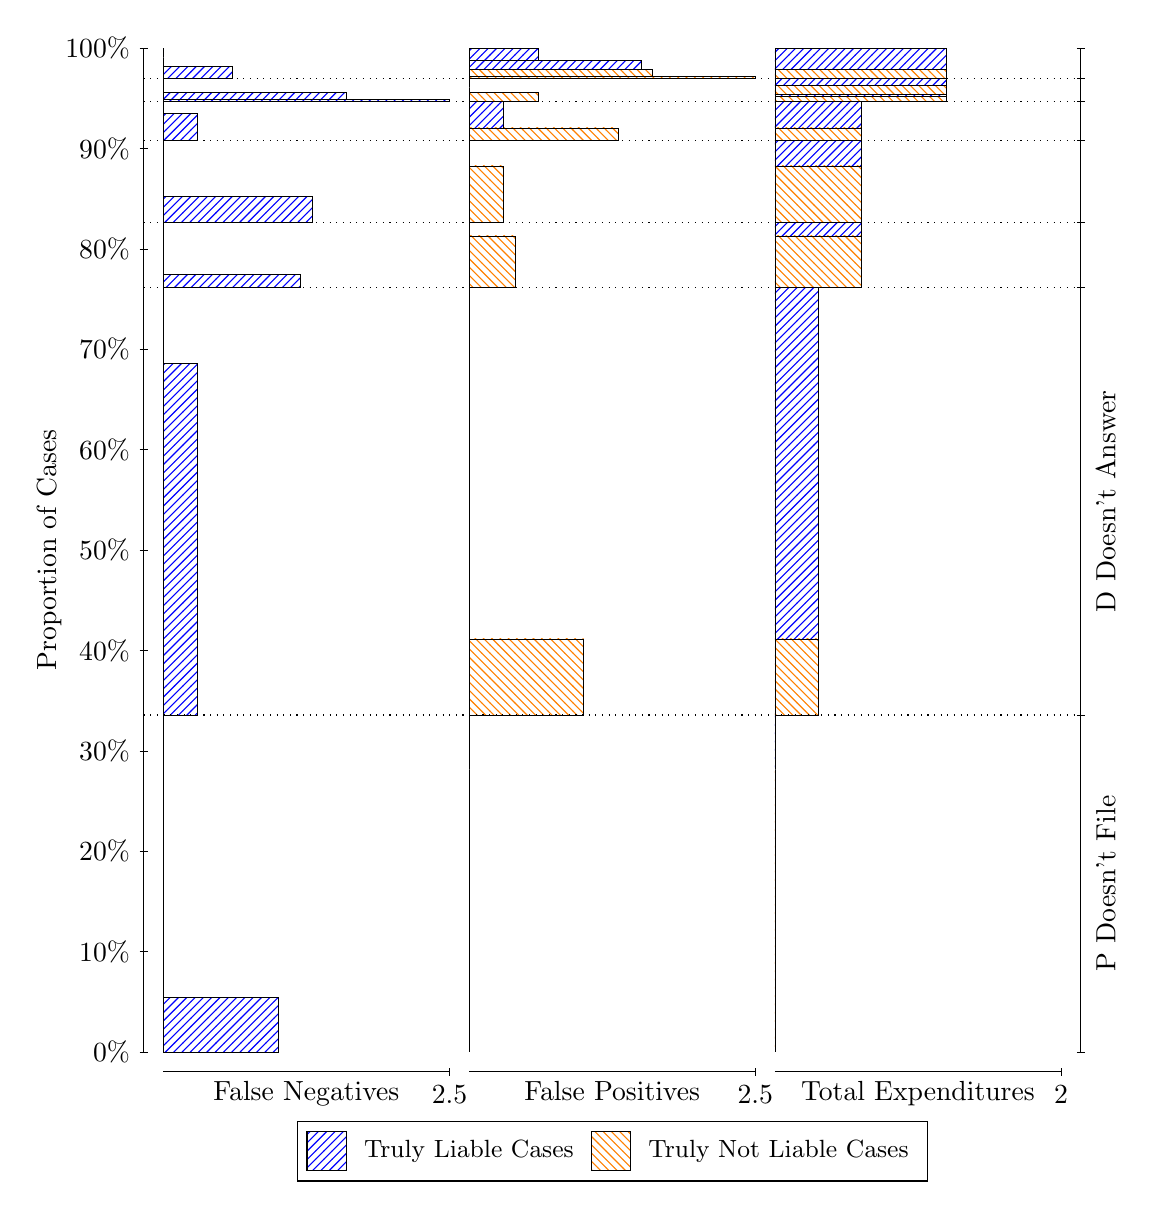
\begin{tikzpicture}
\draw[black, very thin] (1.5,1.75) -- (1.5,14.5);
\node[rotate=90, text=black, anchor=center] at (0.3, 8.125) {Proportion of Cases};
\draw[black, very thin] (1.45,1.75) -- (1.55,1.75);
\node[text=black, anchor=east] at (1.45, 1.75) {0\%};
\draw[black, very thin] (1.45,3.025) -- (1.55,3.025);
\node[text=black, anchor=east] at (1.45, 3.025) {10\%};
\draw[black, very thin] (1.45,4.3) -- (1.55,4.3);
\node[text=black, anchor=east] at (1.45, 4.3) {20\%};
\draw[black, very thin] (1.45,5.575) -- (1.55,5.575);
\node[text=black, anchor=east] at (1.45, 5.575) {30\%};
\draw[black, very thin] (1.45,6.85) -- (1.55,6.85);
\node[text=black, anchor=east] at (1.45, 6.85) {40\%};
\draw[black, very thin] (1.45,8.125) -- (1.55,8.125);
\node[text=black, anchor=east] at (1.45, 8.125) {50\%};
\draw[black, very thin] (1.45,9.4) -- (1.55,9.4);
\node[text=black, anchor=east] at (1.45, 9.4) {60\%};
\draw[black, very thin] (1.45,10.675) -- (1.55,10.675);
\node[text=black, anchor=east] at (1.45, 10.675) {70\%};
\draw[black, very thin] (1.45,11.95) -- (1.55,11.95);
\node[text=black, anchor=east] at (1.45, 11.95) {80\%};
\draw[black, very thin] (1.45,13.225) -- (1.55,13.225);
\node[text=black, anchor=east] at (1.45, 13.225) {90\%};
\draw[black, very thin] (1.45,14.5) -- (1.55,14.5);
\node[text=black, anchor=east] at (1.45, 14.5) {100\%};

\draw[black, very thin] (13.4,1.75) -- (13.4,14.5);
\draw[black, very thin] (13.35,1.75) -- (13.45,1.75);
\node[anchor=west] at (13.35, 1.75) {};
\draw[black, very thin] (13.35,6.0293) -- (13.45,6.0293);
\node[anchor=west] at (13.35, 6.0293) {};
\draw[black, very thin] (13.35,11.457) -- (13.45,11.457);
\node[anchor=west] at (13.35, 11.457) {};
\draw[black, very thin] (13.35,12.286) -- (13.45,12.286);
\node[anchor=west] at (13.35, 12.286) {};
\draw[black, very thin] (13.35,13.331) -- (13.45,13.331);
\node[anchor=west] at (13.35, 13.331) {};
\draw[black, very thin] (13.35,13.823) -- (13.45,13.823);
\node[anchor=west] at (13.35, 13.823) {};
\draw[black, very thin] (13.35,14.114) -- (13.45,14.114);
\node[anchor=west] at (13.35, 14.114) {};
\draw[black, very thin] (13.35,14.5) -- (13.45,14.5);
\node[anchor=west] at (13.35, 14.5) {};

\draw[black, very thin, pattern color=blue, pattern=north east lines] (1.75,1.75) rectangle (3.2033,2.4396);
\draw[black, very thin, pattern color=orange, pattern=north west lines] (1.75,2.4396) rectangle (1.75,6.0293);
\draw[black, very thin, pattern color=blue, pattern=north east lines] (1.75,6.0293) rectangle (2.186,10.491);
\draw[black, very thin, pattern color=orange, pattern=north west lines] (1.75,10.491) rectangle (1.75,11.457);
\draw[black, very thin, pattern color=blue, pattern=north east lines] (1.75,11.457) rectangle (3.494,11.63);
\draw[black, very thin, pattern color=orange, pattern=north west lines] (1.75,11.63) rectangle (1.75,12.286);
\draw[black, very thin, pattern color=blue, pattern=north east lines] (1.75,12.286) rectangle (3.6393,12.615);
\draw[black, very thin, pattern color=orange, pattern=north west lines] (1.75,12.615) rectangle (1.75,13.331);
\draw[black, very thin, pattern color=blue, pattern=north east lines] (1.75,13.331) rectangle (2.186,13.668);
\draw[black, very thin, pattern color=orange, pattern=north west lines] (1.75,13.668) rectangle (1.75,13.823);
\draw[black, very thin, pattern color=blue, pattern=north east lines] (1.75,13.823) rectangle (5.3833,13.846);
\draw[black, very thin, pattern color=blue, pattern=north east lines] (1.75,13.846) rectangle (4.0753,13.936);
\draw[black, very thin, pattern color=orange, pattern=north west lines] (1.75,13.936) rectangle (1.75,14.114);
\draw[black, very thin, pattern color=blue, pattern=north east lines] (1.75,14.114) rectangle (2.622,14.267);
\draw[black, very thin, pattern color=orange, pattern=north west lines] (1.75,14.267) rectangle (1.75,14.38);
\draw[black, very thin, pattern color=blue, pattern=north east lines] (1.75,14.38) rectangle (1.75,14.5);
\draw[black, very thin, pattern color=orange, pattern=north west lines] (5.6333,1.75) rectangle (5.6333,5.3397);
\draw[black, very thin, pattern color=blue, pattern=north east lines] (5.6333,5.3397) rectangle (5.6333,6.0293);
\draw[black, very thin, pattern color=orange, pattern=north west lines] (5.6333,6.0293) rectangle (7.0867,6.9953);
\draw[black, very thin, pattern color=blue, pattern=north east lines] (5.6333,6.9953) rectangle (5.6333,11.457);
\draw[black, very thin, pattern color=orange, pattern=north west lines] (5.6333,11.457) rectangle (6.2147,12.114);
\draw[black, very thin, pattern color=blue, pattern=north east lines] (5.6333,12.114) rectangle (5.6333,12.286);
\draw[black, very thin, pattern color=orange, pattern=north west lines] (5.6333,12.286) rectangle (6.0693,13.003);
\draw[black, very thin, pattern color=blue, pattern=north east lines] (5.6333,13.003) rectangle (5.6333,13.331);
\draw[black, very thin, pattern color=orange, pattern=north west lines] (5.6333,13.331) rectangle (7.5227,13.487);
\draw[black, very thin, pattern color=blue, pattern=north east lines] (5.6333,13.487) rectangle (6.0693,13.823);
\draw[black, very thin, pattern color=orange, pattern=north west lines] (5.6333,13.823) rectangle (6.5053,13.935);
\draw[black, very thin, pattern color=orange, pattern=north west lines] (5.6333,13.935) rectangle (5.6333,14.001);
\draw[black, very thin, pattern color=blue, pattern=north east lines] (5.6333,14.001) rectangle (5.6333,14.114);
\draw[black, very thin, pattern color=orange, pattern=north west lines] (5.6333,14.114) rectangle (9.2667,14.142);
\draw[black, very thin, pattern color=orange, pattern=north west lines] (5.6333,14.142) rectangle (7.9587,14.227);
\draw[black, very thin, pattern color=blue, pattern=north east lines] (5.6333,14.227) rectangle (7.8133,14.346);
\draw[black, very thin, pattern color=blue, pattern=north east lines] (5.6333,14.346) rectangle (6.5053,14.5);
\draw[black, very thin, pattern color=orange, pattern=north west lines] (9.5167,1.75) rectangle (9.5167,5.3397);
\draw[black, very thin, pattern color=blue, pattern=north east lines] (9.5167,5.3397) rectangle (9.5167,6.0293);
\draw[black, very thin, pattern color=orange, pattern=north west lines] (9.5167,6.0293) rectangle (10.062,6.9953);
\draw[black, very thin, pattern color=blue, pattern=north east lines] (9.5167,6.9953) rectangle (10.062,11.457);
\draw[black, very thin, pattern color=orange, pattern=north west lines] (9.5167,11.457) rectangle (10.607,12.114);
\draw[black, very thin, pattern color=blue, pattern=north east lines] (9.5167,12.114) rectangle (10.607,12.286);
\draw[black, very thin, pattern color=orange, pattern=north west lines] (9.5167,12.286) rectangle (10.607,13.003);
\draw[black, very thin, pattern color=blue, pattern=north east lines] (9.5167,13.003) rectangle (10.607,13.331);
\draw[black, very thin, pattern color=orange, pattern=north west lines] (9.5167,13.331) rectangle (10.607,13.487);
\draw[black, very thin, pattern color=blue, pattern=north east lines] (9.5167,13.487) rectangle (10.607,13.823);
\draw[black, very thin, pattern color=orange, pattern=north west lines] (9.5167,13.823) rectangle (11.697,13.889);
\draw[black, very thin, pattern color=blue, pattern=north east lines] (9.5167,13.889) rectangle (11.697,13.912);
\draw[black, very thin, pattern color=orange, pattern=north west lines] (9.5167,13.912) rectangle (11.697,14.024);
\draw[black, very thin, pattern color=blue, pattern=north east lines] (9.5167,14.024) rectangle (11.697,14.114);
\draw[black, very thin, pattern color=orange, pattern=north west lines] (9.5167,14.114) rectangle (11.697,14.227);
\draw[black, very thin, pattern color=blue, pattern=north east lines] (9.5167,14.227) rectangle (11.697,14.5);
\draw[black, dotted] (1.5,6.0293) -- (13.4,6.0293);
\draw[black, dotted] (1.5,11.457) -- (13.4,11.457);
\draw[black, dotted] (1.5,12.286) -- (13.4,12.286);
\draw[black, dotted] (1.5,13.331) -- (13.4,13.331);
\draw[black, dotted] (1.5,13.823) -- (13.4,13.823);
\draw[black, dotted] (1.5,14.114) -- (13.4,14.114);
\draw[black, very thin] (1.75,1.5) -- (5.3833,1.5);
\node[text=black, anchor=north] at (3.5667, 1.5) {False Negatives};
\draw[black, very thin] (5.3833,1.45) -- (5.3833,1.55);
\node[text=black, anchor=north] at (5.3833, 1.45) {2.5};

\draw[black, very thin] (5.6333,1.5) -- (9.2667,1.5);
\node[text=black, anchor=north] at (7.45, 1.5) {False Positives};
\draw[black, very thin] (9.2667,1.45) -- (9.2667,1.55);
\node[text=black, anchor=north] at (9.2667, 1.45) {2.5};

\draw[black, very thin] (9.5167,1.5) -- (13.15,1.5);
\node[text=black, anchor=north] at (11.333, 1.5) {Total Expenditures};
\draw[black, very thin] (13.15,1.45) -- (13.15,1.55);
\node[text=black, anchor=north] at (13.15, 1.45) {2};

\node[text=black, centered, rotate=90] at (13.72, 3.8897) {P Doesn't File};
\node[text=black, centered, rotate=90] at (13.72, 8.7433) {D Doesn't Answer};






\draw (7.449999999999999,1.5) node[draw=none] (baseCoordinate) {};
\begin{scope}[align=center]
        \matrix[scale=0.5, draw=black, below=0.5cm of baseCoordinate, nodes={draw}, column sep=0.1cm]{
            \node[rectangle, draw, minimum width=0.5cm, minimum height=0.5cm, pattern color=blue, pattern=north east lines] {}; &
            \node[draw=none, font=\small, text=black] (B) {Truly Liable Cases}; &
            \node[rectangle, draw, minimum width=0.5cm, minimum height=0.5cm, pattern color=orange, pattern=north west lines] {}; &
            \node[draw=none, font=\small, text=black] (B) {Truly Not Liable Cases}; \\
            };
\end{scope}

\end{tikzpicture}
\end{document}